\documentclass[../../Thesis.tex]{subfiles}
\usepackage[italian]{babel}

\begin{document}
\chapter{Risultati}
\label{chap:results}
Questo capitolo finale del lavoro di tesi \`e dedicato alla valutazione e all'analisi dei risultati ottenuti da tutti gli esperimenti condotti. Nei prossimi paragrafi verr\`a introdotta la struttura del capitolo. 

Inizieremo introducendo le metriche di valutazione utilizzate per misurare le prestazioni dei modelli, cercando di fornire una panoramica delle metriche utilizzate e delle loro applicazioni. 

Successivamente, presenteremo i risultati ottenuti dai modelli di classificazione applicati alla classificazione del bytecode. 
A seguire, verranno illustrati i risultati dei modelli utilizzati per la classificazione del codice sorgente Solidity. In entrambi i casi, verranno presentati i risultati di tutti gli esperimenti nelle varie configurazioni, seguite da un'analisi dei risultati ottenuti.

Dopo aver esaminato i risultati dei modelli sulle diverse modalit\`a in input, presenteremo i risultati ottenuti tramite lo stacking dei modelli. Questa tecnica avanzata, che combina pi\`u modelli per migliorare la precisione e la robustezza delle previsioni, sar\`a discussa in termini di efficacia rispetto ai singoli modelli utilizzati.

Infine, concluderemo con la presentazione dei risultati ottenuti dal modello Gemini di Google. Questa sezione fornir\`a un'analisi critica delle performance del modello Gemini, confrontandole con i risultati ottenuti dai modelli precedenti e valutando il suo contributo complessivo all'interno del contesto della ricerca.

\section{Metriche di Valutazione}

In questo capitolo verranno introdotte le metriche di valutazione utilizzate per analizzare le performance dei modelli implementati. Le metriche di valutazione sono strumenti fondamentali per misurare l'efficacia di un modello di classificazione, confrontando le sue previsioni con le etichette reali del dataset. Le metriche sono calcolate a partire dalle seguenti misurazioni:

\begin{itemize}
\item \textbf{True Positives (TP)}: Il numero di istanze correttamente classificate come appartenenti a una specifica classe.
\item \textbf{True Negatives (TN)}: Il numero di istanze correttamente classificate come non appartenenti a una specifica classe.
\item \textbf{False Positives (FP)}: Il numero di istanze erroneamente classificate come appartenenti a una specifica classe.
\item \textbf{False Negatives (FN)}: Il numero di istanze erroneamente classificate come non appartenenti a una specifica classe.
\end{itemize}

Queste misurazioni costituiscono la base per il calcolo delle diverse metriche di valutazione, che forniscono una visione dettagliata delle prestazioni del modello in vari aspetti chiave.

\subsection{Accuracy}
L'accuracy misura la proporzione degli esempi che sono stati correttamente classificati. Pi\`u precisamente, \`e la somma dei true positives e dei true negatives diviso per il numero totale di istanze. La formula per il calcolo dell'accuracy \`e la seguente:
$$ \text{Accuracy} = \frac{TP + TN}{TP + TN + FP + FN} $$
L'accuracy \`e semplice da interpretare e calcolare, specialmente in contesti di classificazione binaria. Tuttavia, in contesti di classificazione multilabel con classi sbilanciate, pu\`o risultare fuorviante poich\`e non considera la distribuzione delle classi.

Ad esempio, in un problema di classificazione multilabel dove ciascuna istanza pu\`o appartenere a pi\`u classi contemporaneamente, consideriamo un dataset con le seguenti distribuzioni: il 70\% delle istanze appartiene alla classe A, il 20\% alla classe B, e il 10\% alla classe C. Un modello che classifica tutte le istanze come appartenenti solo alla classe A potrebbe ottenere un'accuracy elevata, ignorando completamente le classi B e C. Questo risultato non rifletterebbe adeguatamente la capacit\`a del modello di gestire tutte le classi presenti. 

Pertanto, sebbene l'accuracy possa fornire una misura rapida delle performance di un modello, \`e importante considerarla insieme ad altre metriche di valutazione, come precision, recall e F1-score, specialmente in contesti di classificazione multilabel, per ottenere una visione pi\`u completa e accurata delle capacit\`a del modello.

\subsection{Precision}
La Precision misura la proporzione di predizioni corrette tra tutte le predizioni di una certa classe. In altre parole \`e la proporzione dei true positive rispetto a tutte le predizioni positive.
$$Precision = \frac{ TP}{ TP + FP} $$
In un contesto di classificazione multilabel, la precision pu\`o essere calcolata in tre modi differenti:

\begin{itemize}
    \item \textbf{Micro Precision}: Aggrega i contributi di tutte le classi per calcolare la precision complessiva.
    $$ \text{Micro Precision} = \frac{\sum TP}{\sum TP + \sum FP} $$
    \item \textbf{Macro Precision}: Calcola la precision per ogni classe e poi ne fa la media.
    $$ \text{Macro Precision} = \frac{1}{N} \sum_{i=1}^{N} \text{Precision}_i $$
    \item \textbf{Weighted Precision}: Calcola la precision per ogni classe ponderata per il numero di veri positivi.
    $$ \text{Weighted Precision} = \frac{\sum_{i=1}^{N} \text{Precision}_i \times w_i}{\sum_{i=1}^{N} w_i} $$
\end{itemize}
La precision ha il vantaggio che indica quanto rilevanti siano le previsioni fatte, cio\`e la proporzione di istanze classificate correttamente tra quelle classificate come positive. In contesti in cui \`e importante evitare falsi positivi la precision \`e una metrica molto utile. Al contrario, se il modello ha pochi falsi positivi ma molti falsi negativi, la precisio pu\`o essere ingannevole. La precision non \`e molto utile se considerata isolatamente, poich\`e non rifletta la capacit\`a del modello di identificare tutte le istanze rilevanti.

\subsection{Recall}
La Recall misura la proporzione di istanze rilevanti che sono state recuperate. Di conseguenza, \`e la proporzione dei veri positivi su tutti i positivi.
$$Recall = \frac{ TP}{TP + FN} $$
Anche la Recall, come la precision, in un contesto multilabel pu\`o essere calcolata in tre modi differenti:
\begin{itemize}
    \item \textbf{Micro Recall}: Aggrega i contributi di tutte le classi per calcolare la recall complessiva.
    $$ \text{Micro Recall} = \frac{\sum TP}{\sum TP + \sum FN} $$
    \item \textbf{Macro Recall}: Calcola la recall per ogni classe e poi ne fa la media.
    $$ \text{Macro Recall} = \frac{1}{N} \sum_{i=1}^{N} \text{Recall}_i $$
    \item \textbf{Weighted Recall}: Calcola la recall per ogni classe ponderata per il numero di veri positivi.
    $$ \text{Weighted Recall} = \frac{\sum_{i=1}^{N} \text{Recall}_i \times w_i}{\sum_{i=1}^{N} w_i} $$
\end{itemize}
A differenza delle Precision, la recall indica quanto bene il modello riesce a identificare tutte le istanze rilevanti di una classe, cio\`e la proporzione di veri positivi tra tutte le istanze che avrebbero dovuto essere classificate come positive. La recall \`e particolarmente utile in contesti in cui \`e importante evitare falsi negativi, come il rilevamento di malattie o, come nel nostro caso, la rilevazione delle vulnerabilit\`a all'interno degli Smart Contracts. Tuttavia, la recall non \`e molto utile se considerata isolatamente, poich\`e non riflette la capacit\`a del modello di evitare falsi positivi.

\subsection{F1 Score}
L'F1-score \`e la media armonica della precision e della recall, ed \`e utilizzato per trovare un equilibrio tra queste due metriche, soprattutto in contesti con classi sbilanciate. 
$$ F1 = 2 \times \frac{Precision \times Recall}{Precision + Recall} $$
Nella classificazione multilabel, l'F1-score pu\`o essere calcolato in tre modi distinti: Micro, Macro e Weighted. 

\begin{itemize}
    \item \textbf{Micro F1}: Combina micro precision e micro recall.
    $$ \text{Micro F1} = 2 \times \frac{\text{Micro Precision} \times \text{Micro Recall}}{\text{Micro Precision} + \text{Micro Recall}} $$
    \item \textbf{Macro F1}: Calcola l'F1 score per ogni classe e poi ne fa la media.
    $$ \text{Macro F1} = \frac{1}{N} \sum_{i=1}^{N} \text{F1}_i $$
    \item \textbf{Weighted F1}: Calcola l'F1 score per ogni classe ponderata per il numero di veri positivi.
    $$ \text{Weighted F1} = \frac{\sum_{i=1}^{N} \text{F1}_i \times w_i}{\sum_{i=1}^{N} w_i} $$
\end{itemize}
Il grande vantaggio dell'F1 score \`e quello di integrare sia la precision che la recall, offrendo una misura bilanciata delle perfonace del modello, che \`e particolamente utile quando si ha un compromesso tra queste due metriche. L'F1 score \`e particolarmente utile in contesti in cui le classi sono sbilanciate, poich\`e considera sia i falsi positivi che i falsi negativi.
Di contro, l'F1 score pu\`o essere meno interpretabile rispetto alla precision e alla recall, poich\`e offrendo un compromesso tra le due non rende chiaro su quale delle due il modello eccelle e su quale fallisce. Inoltre, in contesti con necessit\`a specifiche come minimizzare i falsi negativi (dando priorit\`a alla recall) o minimizzare i falsi positivi (dando priorit\`a alla precision), l'F1 score potrebbe non fornire l'informazione pi\`u rilevante.

In conclusione, in questo lavoro di tesi, verranno prese in considerazione tutte le metriche sopra descritte, ma, data la natura del problema, poich\`e avere falsi negativi \`e molto pi\`u grave che avere falsi positivi, verr\`a data maggiore importanza alla recall rispetto alla precision. 

 
\section{Risultati modelli sul Bytecode}
In questa sezione verranno presentati i risultati ottenuti dai modelli di classificazione utilizzati per la classificazione del bytecode. I modelli sono stati allenati sul dataset di training, validati sul dataset di validazione e testati sul dataset di test. Le metriche di valutazione, descritte nelle sezioni precedenti, sono state utilizzate per calcolare le prestazioni dei modelli.

Per la classificazione del bytecode, inizialmente sono stati utilizzati due modelli: BERT e CodeBERT, con in input ls sequenza massima di 512 token. Dopo aver confrontato i risultati, il modello CodeBERT ha dimostrato prestazioni superiori rispetto al modello BERT. Di conseguenza, CodeBERT \`e stato scelto per gli esperimenti successivi.
\subsection{BERT}
L'accuratezza del modello \`e del 70,48\%. Di seguito il classification report del modello:
\begin{table}[H]
\centering
\small
\begin{tabular}{lcccc}
\hline
\textbf{Class} & \textbf{Precision} & \textbf{Recall} & \textbf{F1-Score} & \textbf{Support} \\
\hline
access-control & 0.87 & 0.67 & 0.76 & 2331 \\
arithmetic & 0.88 & 0.59 & 0.71 & 2708 \\
other & 0.81 & 0.73 & 0.76 & 4193 \\
reentrancy & 0.88 & 0.78 & 0.83 & 4838 \\
unchecked-calls & 0.90 & 0.87 & 0.88 & 7276 \\
\hline
\textbf{Micro avg} & 0.8726 & 0.7654 & 0.8155 & 21346 \\
\textbf{Macro avg} & 0.8694 & 0.7287 & 0.7895 & 21346 \\
\textbf{Weighted avg} & 0.8724 & 0.7654 & 0.8126 & 21346 \\
\hline
\end{tabular}
\caption{Classification Report del modello BERT sul bytecode}
\end{table}

\subsection{CodeBert}

L'accuratezza del modello \`e del 72,54\%. Di seguito il classification report del modello: 
\begin{table}[H]
\centering
\small
\begin{tabular}{lcccc}
\hline
\textbf{Class} & \textbf{Precision} & \textbf{Recall} & \textbf{F1-Score} & \textbf{Support} \\
\hline
access-control & 0.87 & 0.72 & 0.79 & 2331 \\
arithmetic & 0.81 & 0.69 & 0.75 & 2708 \\
other & 0.85 & 0.73 & 0.78 & 4193 \\
reentrancy & 0.88 & 0.81 & 0.84 & 4838 \\
unchecked-calls & 0.93 & 0.86 & 0.89 & 7276 \\
\hline
\textbf{Micro avg} & 0.8800 & 0.7869 & 0.8309 & 21346 \\
\textbf{Macro avg} & 0.8661 & 0.7622 & 0.8104 & 21346 \\
\textbf{Weighted avg} & 0.8787 & 0.7869 & 0.8298 & 21346 \\
\hline
\end{tabular}
\caption{Classification Report del modello CodeBert sul bytecode}
\end{table}

\subsection{CodeBert Aggregazione di due chunk}
\subsubsection{Aggregazione con funzione Mean}
L'accuratezza del modello \`e del 76.13\%. Di seguito il classification report del modello:
\begin{table}[H]
    \centering
    \small
    \begin{tabular}{lcccc}
    \hline
    \textbf{Class} & \textbf{Precision} & \textbf{Recall} & \textbf{F1-Score} & \textbf{Support} \\
    \hline
    access-control & 0.88 & 0.77 & 0.82 & 2331 \\
    arithmetic & 0.82 & 0.76 & 0.79 & 2708 \\
    other & 0.86 & 0.78 & 0.82 & 4193 \\
    reentrancy & 0.89 & 0.84 & 0.86 & 4838 \\
    unchecked-calls & 0.91 & 0.91 & 0.91 & 7276 \\
    \hline
    \textbf{Micro avg} & 0.8805 & 0.8349 & 0.8571 & 21346 \\
    \textbf{Macro avg} & 0.8708 & 0.8121 & 0.8400 & 21346 \\
    \textbf{Weighted avg} & 0.8795 & 0.8349 & 0.8561 & 21346 \\
    \hline
    \end{tabular}
    \caption{Classification Report per il modello CodeBERT sul bytecode con aggregazione a due chunk usando la media}
    \end{table}
    
    

\subsubsection{Aggregazione con funzione Max}
L'accuratezza del modello \`e del 76.10\%. Di seguito il classification report del modello:
\begin{table}[H]
    \centering
    \small
    \begin{tabular}{lcccc}
    \hline
    \textbf{Class} & \textbf{Precision} & \textbf{Recall} & \textbf{F1-Score} & \textbf{Support} \\
    \hline
    access-control & 0.85 & 0.78 & 0.81 & 2331 \\
    arithmetic & 0.86 & 0.73 & 0.79 & 2708 \\
    other & 0.83 & 0.82 & 0.82 & 4193 \\
    reentrancy & 0.87 & 0.86 & 0.86 & 4838 \\
    unchecked-calls & 0.90 & 0.93 & 0.92 & 7276 \\
    \hline
    \textbf{Micro avg} & 0.8691 & 0.8513 & 0.8601 & 21346 \\
    \textbf{Macro avg} & 0.8612 & 0.8245 & 0.8415 & 21346 \\
    \textbf{Weighted avg} & 0.8682 & 0.8513 & 0.8588 & 21346 \\
    \hline
    \end{tabular}
    \caption{Classification Report per il modello codeBERT sul bytecode con aggregazione a due chunk usando il massimo}
    \end{table}

\subsection{CodeBert Aggregazione di tre chunk}
    \subsubsection{Aggregazione con funzione Mean}
    L'accuratezza del modello \`e del 76.75\%. Di seguito il classification report del modello:
    
    \begin{table}[H]
        \centering
        \small
        \begin{tabular}{lcccc}
        \hline
        \textbf{Class} & \textbf{Precision} & \textbf{Recall} & \textbf{F1-Score} & \textbf{Support} \\
        \hline
        access-control & 0.86 & 0.78 & 0.82 & 2331 \\
        arithmetic & 0.81 & 0.77 & 0.79 & 2708 \\
        other & 0.82 & 0.83 & 0.82 & 4193 \\
        reentrancy & 0.88 & 0.86 & 0.87 & 4838 \\
        unchecked-calls & 0.92 & 0.92 & 0.92 & 7276 \\
        \hline
        \textbf{Micro avg} & 0.8725 & 0.8530 & 0.8626 & 21346 \\
        \textbf{Macro avg} & 0.8590 & 0.8302 & 0.8440 & 21346 \\
        \textbf{Weighted avg} & 0.8722 & 0.8530 & 0.8622 & 21346 \\
        \hline
        \end{tabular}
        \caption{Classification Report per CodeBERT sul bytecode con aggregazione a tre chunk usando la media}
    \end{table}
        
        
    
\subsubsection{Aggregazione con funzione Max}
L'accuratezza del modello \`e del 76.60\%. Di seguito il classification report del modello:
\begin{table}[H]
\centering
\small
\begin{tabular}{lcccc}
\hline
\textbf{Class} & \textbf{Precision} & \textbf{Recall} & \textbf{F1-Score} & \textbf{Support} \\
\hline
access-control & 0.83 & 0.80 & 0.82 & 2331 \\
arithmetic & 0.85 & 0.74 & 0.79 & 2708 \\
other & 0.84 & 0.82 & 0.83 & 4193 \\
reentrancy & 0.89 & 0.84 & 0.86 & 4838 \\
unchecked-calls & 0.92 & 0.92 & 0.92 & 7276 \\
\hline
\textbf{Micro avg} & 0.8796 & 0.8462 & 0.8626 & 21346 \\
\textbf{Macro avg} & 0.8659 & 0.8242 & 0.8441 & 21346 \\
\textbf{Weighted avg} & 0.8789 & 0.8462 & 0.8619 & 21346 \\
\hline
\end{tabular}
\caption{Classification Report per CodeBERT con aggregazione a tre chunk usando il massimo}
\end{table}
\begin{figure}[H]
    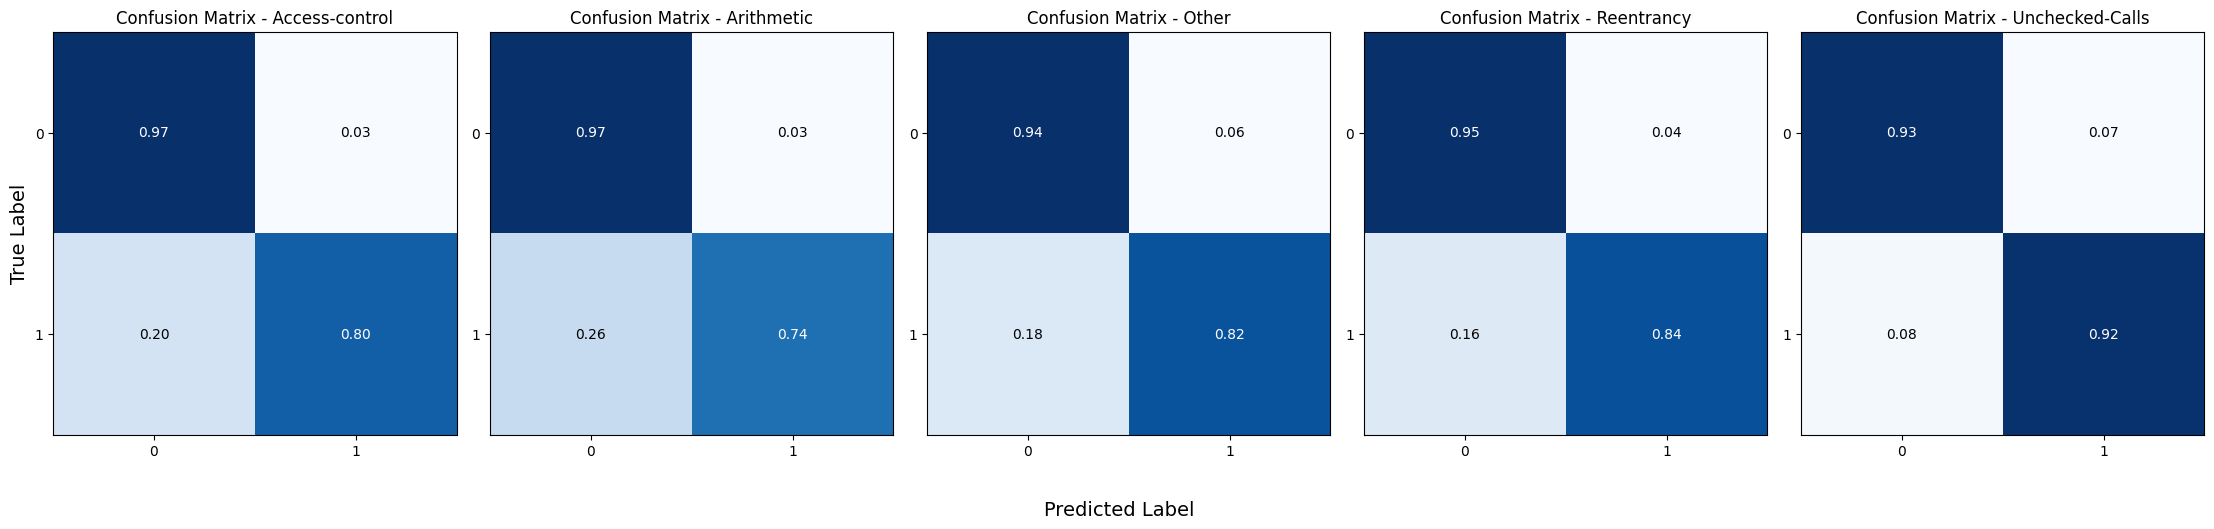
\includegraphics[width=1.05\textwidth]{../../img/CFMax3-BC.png}
    \caption{Confusion Matrices per le diverse classi del modello CodeBERT con aggregazione di tre chunk usando la funzione max sul bytecode}
\end{figure}

\subsection{CodeBERT con Concatenazione}
\subsubsection{CodeBert Concatenazione di due chunk}
L'accuratezza del modello \`e del 76,26\%. Di seguito il classification report del modello:

\begin{table}[H]
    \centering
    \small
    \begin{tabular}{lcccc}
    \hline
    \textbf{Class} & \textbf{Precision} & \textbf{Recall} & \textbf{F1-Score} & \textbf{Support} \\
    \hline
    access-control & 0.86 & 0.78 & 0.82 & 2331 \\
    arithmetic & 0.82 & 0.76 & 0.79 & 2708 \\
    other & 0.84 & 0.81 & 0.83 & 4193 \\
    reentrancy & 0.89 & 0.85 & 0.87 & 4838 \\
    unchecked-calls & 0.90 & 0.93 & 0.91 & 7276 \\
    \hline
    \textbf{Micro avg} & 0.8725 & 0.8487 & 0.8604 & 21346 \\
    \textbf{Macro avg} & 0.8619 & 0.8250 & 0.8427 & 21346 \\
    \textbf{Weighted avg} & 0.8715 & 0.8487 & 0.8596 & 21346 \\
    \hline
    \end{tabular}
    \caption{Classification Report per CodeBERT con concatenazione di due chunk}
    \end{table}
\subsubsection{CodeBert Concatenazione di tre chunk}
L'accuratezza del modello \`e del 76.80\%. Di seguito il classification report del modello:

\begin{table}[H]
    \centering
    \small
    \begin{tabular}{lcccc}
    \hline
    \textbf{Class} & \textbf{Precision} & \textbf{Recall} & \textbf{F1-Score} & \textbf{Support} \\
    \hline
    access-control & 0.84 & 0.79 & 0.82 & 2331 \\
    arithmetic & 0.87 & 0.73 & 0.80 & 2708 \\
    other & 0.84 & 0.81 & 0.83 & 4193 \\
    reentrancy & 0.90 & 0.84 & 0.87 & 4838 \\
    unchecked-calls & 0.92 & 0.92 & 0.92 & 7276 \\
    \hline
    \textbf{Micro avg} & 0.8862 & 0.8435 & 0.8643 & 21346 \\
    \textbf{Macro avg} & 0.8749 & 0.8197 & 0.8457 & 21346 \\
    \textbf{Weighted avg} & 0.8856 & 0.8435 & 0.8634 & 21346 \\
    \hline
    \end{tabular}
    \caption{Classification Report per il modello CodeBERT concatenando tre chunk}
\end{table}

\begin{figure}[h!]
    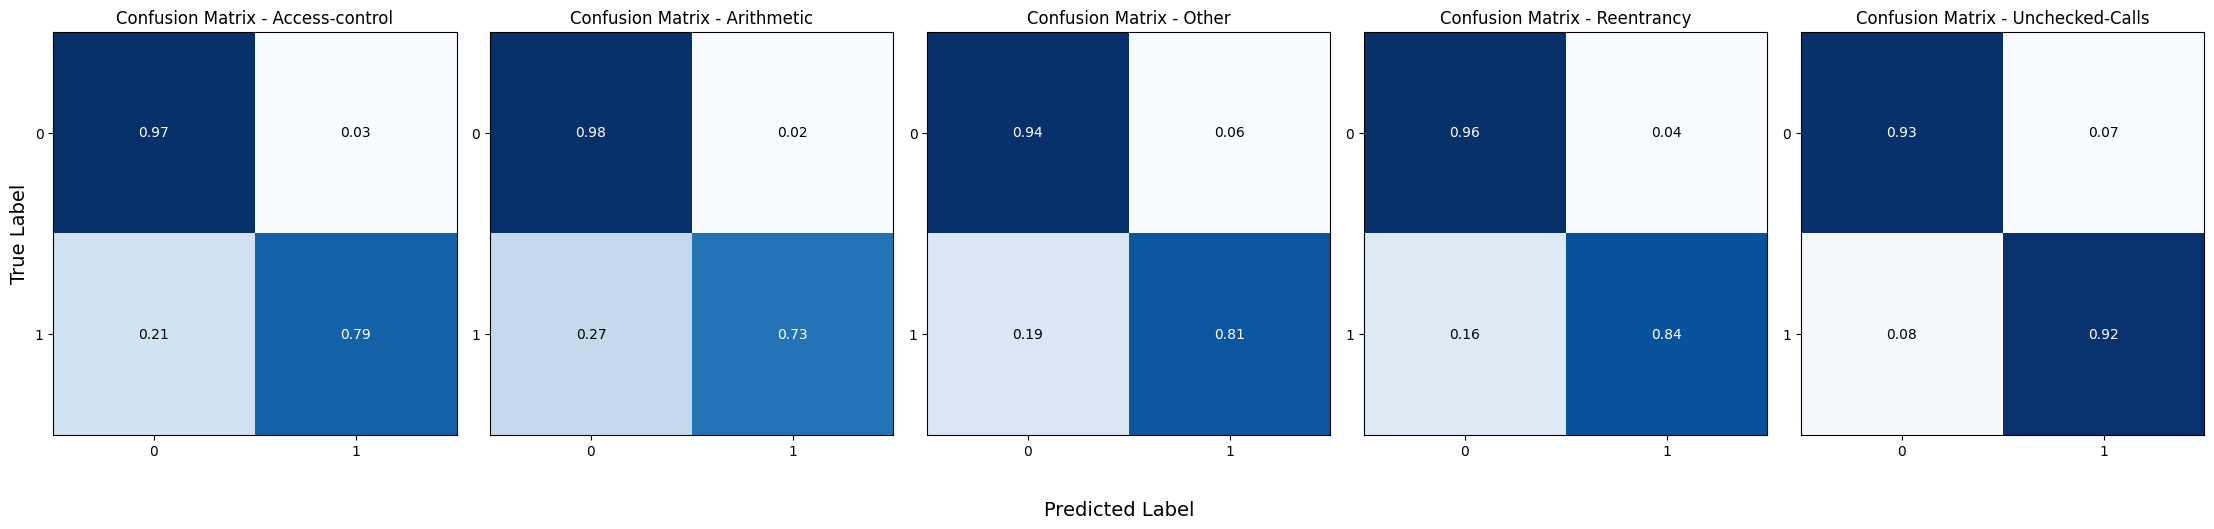
\includegraphics[width=1.05\textwidth]{../../img/CFConcat3-BC.png}
    \caption{Confusion Matrices per le diverse classi del modello CodeBERT con concatenazione di tre chunk sul bytecode}
\end{figure}

\subsection{Analisi}
Per i modelli allenati sul bytecode, i risultati migliori, sugli esperimenti iniziali utilizzando un blocco di codice da 512 token per la classificazione, sono stati ottenuti utilizzando il modello CodeBERT, che ha superato il modello BERT in tutte le metriche di valutazione, eccetto per la recall della classe ``unchecked-calls". Di conseguenza, \`e stato utilizzato il modello CodeBERT per le ulteriori analisi, poich\`e \`e stato quello con le migliori performance.

Successivamente, si \`e esaminato l'effetto dell'aumento del numero di chunk da due a tre. Tuttavia, non si \`e osservato un miglioramento significativo delle prestazioni del modello con il passaggio da due a tre chunk di codice. Il miglior modello, seppur con un vantaggio di pochi decimi, \`e stato quello che ha utilizzato la concatenazione di tre chunk, raggiungendo un'accuratezza del 76,80\% e un F1 Micro dell'86,43\% sul test set.

Analizzando, per\`o, le performance per le singole classi, si \`e osservato che il miglior modello in termini di accuratezza non ha ottenuto le migliori performance in termini di recall per nessuna classe specifica. In dettaglio:
\begin{itemize}
    \item Per la classe ``arithmetic", la miglior performance in termini di recall \`e stata offerta dal modello con aggregazione di tre chunk utilizzando la funzione di media (mean).
    \item Per le restanti classi, il miglior modello in termini di recall \`e stato quello con aggregazione di tre chunk utilizzando la funzione massima (max).
\end{itemize}
Poich\`e la metrica di valutazione pi\`u importante per il nostro problema \`e la recall, il modello con aggregazione di tre chunk utilizzando la funzione max \`e stato scelto come il miglior modello per la classificazione del bytecode.


\section{Risultati sul Codice Sorgente Solidity}

Questa sezione presenta i risultati ottenuti dai modelli di classificazione applicati al codice sorgente Solidity. Anche in questo caso, i modelli sono stati allenati sul dataset di training, validati sul dataset di validazione e testati sul dataset di test. I risultati sono stati valutati utilizzando le metriche di valutazione precedentemente descritte.

Analogamente al bytecode, sono stati inizialmente utilizzati un modello BERT e un modello CodeBERT per la classificazione del codice sorgente Solidity, impiegando 512 token in input. Successivamente, poich\`e anche in questo caso i migliori risultati sono stati ottenuti con il modello CodeBERT, questo \`e stato utilizzato per gli esperimenti successivi, che prevedevano l'uso di porzioni pi\`u ampie dei dati disponibili.
\subsection{BERT}
L'accuratezza del modello \`e del 70.46\%. Di seguito il classification report del modello:
\begin{table}[H]
    \centering
    \small
    \begin{tabular}{lcccc}
    \hline
    \textbf{Class} & \textbf{Precision} & \textbf{Recall} & \textbf{F1-Score} & \textbf{Support} \\
    \hline
    access-control & 0.82 & 0.60 & 0.69 & 2346 \\
    arithmetic & 0.79 & 0.73 & 0.76 & 2715 \\
    other & 0.79 & 0.71 & 0.75 & 4209 \\
    reentrancy & 0.87 & 0.77 & 0.82 & 4846 \\
    unchecked-calls & 0.91 & 0.88 & 0.89 & 7289 \\
    \hline
    \textbf{Micro avg} & 0.8568 & 0.7702 & 0.8112 & 21405 \\
    \textbf{Macro avg} & 0.8384 & 0.7370 & 0.7828 & 21405 \\
    \textbf{Weighted avg} & 0.8550 & 0.7702 & 0.8093 & 21405 \\
    \hline
    \end{tabular}
    \caption{Classification Report per il modello BERT sul codice sorgente Solidity}
\end{table}
\subsection{CodeBert}
\begin{table}[H]
    \centering
    \small
    \begin{tabular}{lcccc}
    \hline
    \textbf{Class} & \textbf{Precision} & \textbf{Recall} & \textbf{F1-Score} & \textbf{Support} \\
    \hline
    access-control & 0.81 & 0.74 & 0.77 & 2346 \\
    arithmetic & 0.81 & 0.77 & 0.79 & 2715 \\
    other & 0.78 & 0.76 & 0.77 & 4209 \\
    reentrancy & 0.88 & 0.81 & 0.84 & 4846 \\
    unchecked-calls & 0.91 & 0.91 & 0.91 & 7289 \\
    \hline
    \textbf{Micro avg} & 0.8563 & 0.8199 & 0.8377 & 21405 \\
    \textbf{Macro avg} & 0.8391 & 0.7969 & 0.8172 & 21405 \\
    \textbf{Weighted avg} & 0.8558 & 0.8199 & 0.8372 & 21405 \\
    \hline
    \end{tabular}
    \caption{Classification Report per il modello di CodeBERT}
    \end{table}
\subsection{DistilBert}
L'accuratezza del modello \`e del 70.35\%. Di seguito il classification report del modello:

\begin{table}[H]
    \centering
    \small
    \begin{tabular}{lcccc}
    \hline
    \textbf{Class} & \textbf{Precision} & \textbf{Recall} & \textbf{F1-Score} & \textbf{Support} \\
    \hline
    access-control & 0.82 & 0.60 & 0.69 & 2346 \\
    arithmetic & 0.79 & 0.71 & 0.75 & 2715 \\
    other & 0.78 & 0.72 & 0.75 & 4209 \\
    reentrancy & 0.86 & 0.78 & 0.81 & 4846 \\
    unchecked-calls & 0.91 & 0.88 & 0.89 & 7289 \\
    \hline
    \textbf{Micro avg} & 0.8487 & 0.7734 & 0.8093 & 21405 \\
    \textbf{Macro avg} & 0.8308 & 0.7378 & 0.7799 & 21405 \\
    \textbf{Weighted avg} & 0.8466 & 0.7734 & 0.8072 & 21405 \\
    \hline
    \end{tabular}
    \caption{Classification Report per il modello DistilBert sul codice sorgente}
\end{table}

\subsection{CodeBERT con concatenazione}
\subsubsection{CodeBert Concatenazione di due chunk}
L'accuratezza del modello \`e del 76,36\%. Di seguito il classification report del modello:

\begin{table}[H]
\centering
\small
\begin{tabular}{lcccc}
\hline
\textbf{Class} & \textbf{Precision} & \textbf{Recall} & \textbf{F1-Score} & \textbf{Support} \\
\hline
access-control & 0.86 & 0.78 & 0.82 & 2331 \\
arithmetic & 0.81 & 0.81 & 0.81 & 2708 \\
other & 0.82 & 0.78 & 0.80 & 4193 \\
reentrancy & 0.90 & 0.80 & 0.85 & 4838 \\
unchecked-calls & 0.94 & 0.91 & 0.93 & 7276 \\
\hline
\textbf{Micro avg} & 0.8819 & 0.8342 & 0.8574 & 21346 \\
\textbf{Macro avg} & 0.8662 & 0.8172 & 0.8406 & 21346 \\
\textbf{Weighted avg} & 0.8821 & 0.8342 & 0.8571 & 21346 \\
\hline
\end{tabular}
\caption{Classification Report del modello CodeBERT con concatenazione di due chunk}
\end{table}
\subsubsection{CodeBert Concatenazione di tre chunk}
L'accuratezza del modello \`e del 79,39\%. Di seguito il classification report del modello:

\begin{table}[H]
\centering
\small
\begin{tabular}{lcccc}
\hline
\textbf{Class} & \textbf{Precision} & \textbf{Recall} & \textbf{F1-Score} & \textbf{Support} \\
\hline
access-control & 0.87 & 0.82 & 0.84 & 2331 \\
arithmetic & 0.90 & 0.81 & 0.85 & 2708 \\
other & 0.87 & 0.79 & 0.83 & 4193 \\
reentrancy & 0.91 & 0.84 & 0.87 & 4838 \\
unchecked-calls & 0.95 & 0.93 & 0.94 & 7276 \\
\hline
\textbf{Micro avg} & 0.9103 & 0.8561 & 0.8824 & 21346 \\
\textbf{Macro avg} & 0.8994 & 0.8387 & 0.8677 & 21346 \\
\textbf{Weighted avg} & 0.9093 & 0.8561 & 0.8816 & 21346 \\
\hline
\end{tabular}
\caption{Classification Report del modello CodeBERT con concatenazione di tre chunk}
\end{table}

\begin{figure}[H]
    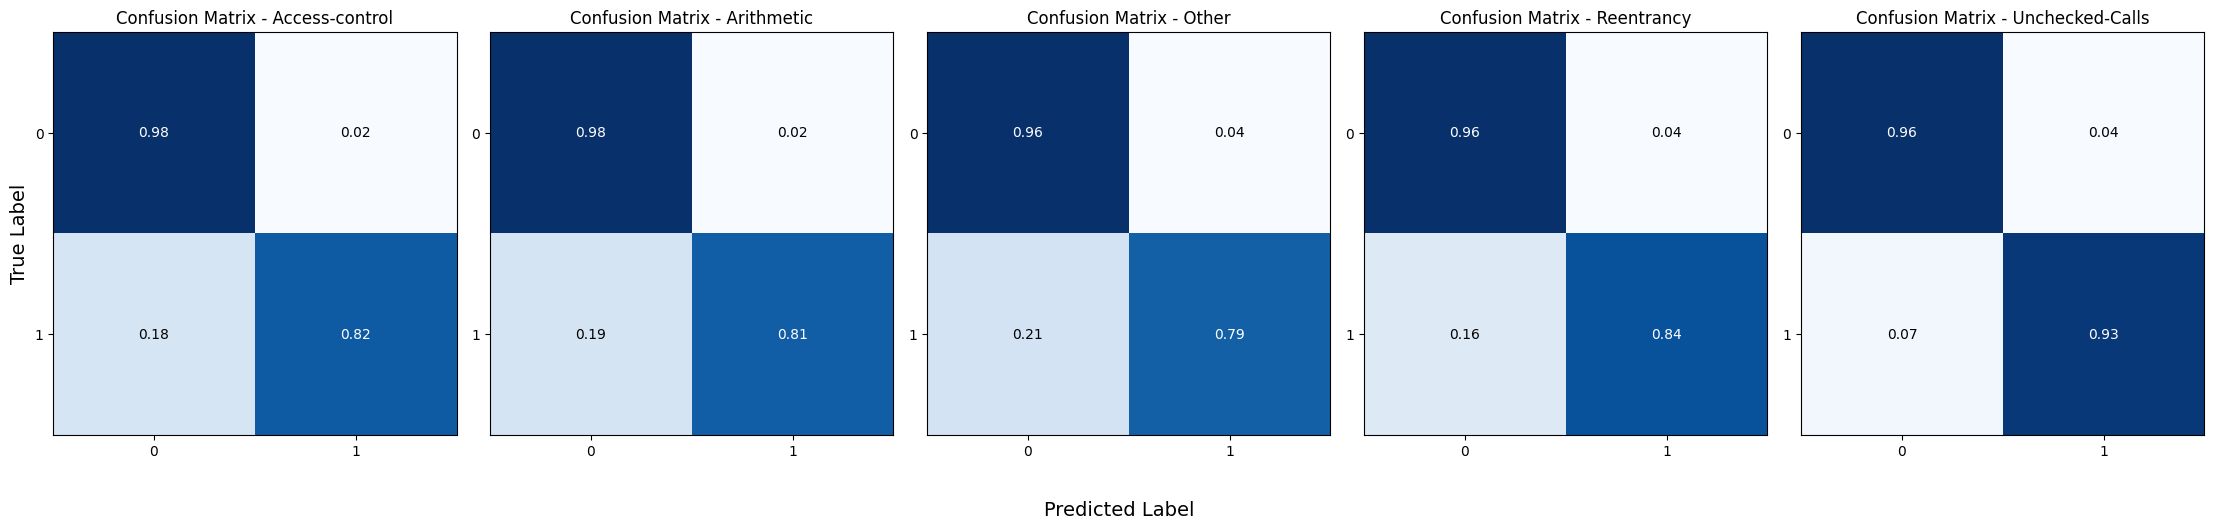
\includegraphics[width=1.05\textwidth]{../../img/CFConcat3-SC.png}
    \caption{Confusion Matrices per le diverse classi del modello CodeBERT con concatenazione di tre chunk sul codice sorgente Solidity}
\end{figure}

\subsection{CodeBert Aggregazione di due chunk}
\subsubsection{Aggregazione con funzione Max}
L'accuratezza del modello \`e del 76.50\%. Di seguito il classification report del modello:

\begin{table}[H]
    \centering
    \small
    \begin{tabular}{lcccc}
    \hline
    \textbf{Class} & \textbf{Precision} & \textbf{Recall} & \textbf{F1-Score} & \textbf{Support} \\
    \hline
    access-control & 0.87 & 0.77 & 0.82 & 2331 \\
    arithmetic & 0.83 & 0.80 & 0.82 & 2708 \\
    other & 0.80 & 0.80 & 0.80 & 4193 \\
    reentrancy & 0.90 & 0.81 & 0.85 & 4838 \\
    unchecked-calls & 0.94 & 0.91 & 0.93 & 7276 \\
    \hline
    \textbf{Micro avg} & 0.8816 & 0.8369 & 0.8586 & 21346 \\
    \textbf{Macro avg} & 0.8687 & 0.8181 & 0.8422 & 21346 \\
    \textbf{Weighted avg} & 0.8821 & 0.8369 & 0.8585 & 21346 \\
    \hline
    \end{tabular}
    \caption{Classification Report del modello codeBERT con aggregazione di due chunk}
    \end{table}

\subsubsection{Aggregazione con funzione Mean}
L'accuratezza del modello \`e del 75.84\%. Di seguito il classification report del modello:
\begin{table}[H]
    \centering
    \small
    \begin{tabular}{lcccc}
    \hline
    \textbf{Class} & \textbf{Precision} & \textbf{Recall} & \textbf{F1-Score} & \textbf{Support} \\
    \hline
    access-control & 0.84 & 0.77 & 0.81 & 2331 \\
    arithmetic & 0.82 & 0.80 & 0.81 & 2708 \\
    other & 0.81 & 0.77 & 0.79 & 4193 \\
    reentrancy & 0.90 & 0.80 & 0.85 & 4838 \\
    unchecked-calls & 0.94 & 0.90 & 0.92 & 7276 \\
    \hline
    \textbf{Micro avg} & 0.8830 & 0.8233 & 0.8521 & 21346 \\
    \textbf{Macro avg} & 0.8657 & 0.8068 & 0.8350 & 21346 \\
    \textbf{Weighted avg} & 0.8833 & 0.8233 & 0.8520 & 21346 \\
    \hline
    \end{tabular}
    \caption{Classification Report del modello CodeBERT con aggregazione di due chunk}
    \end{table}


    
\subsection{CodeBert Aggregazione di tre chunk}
\subsubsection{Aggregazione con funzione Max}
L'accuratezza del modello \`e del 79.08\%. Di seguito il classification report del modello:
\begin{table}[H]
    \centering
    \small
    \begin{tabular}{lcccc}
    \hline
    \textbf{Class} & \textbf{Precision} & \textbf{Recall} & \textbf{F1-Score} & \textbf{Support} \\
    \hline
    access-control & 0.87 & 0.83 & 0.85 & 2331 \\
    arithmetic & 0.86 & 0.84 & 0.85 & 2708 \\
    other & 0.84 & 0.82 & 0.83 & 4193 \\
    reentrancy & 0.91 & 0.84 & 0.87 & 4838 \\
    unchecked-calls & 0.95 & 0.94 & 0.94 & 7276 \\
    \hline
    \textbf{Micro avg} & 0.8983 & 0.8671 & 0.8824 & 21346 \\
    \textbf{Macro avg} & 0.8855 & 0.8524 & 0.8685 & 21346 \\
    \textbf{Weighted avg} & 0.8983 & 0.8671 & 0.8822 & 21346 \\
    \hline
    \end{tabular}
    \caption{Classification Report del modello con aggregazione di tre chunk usando la funzione Max}
    \end{table}

    \begin{figure}[H]
        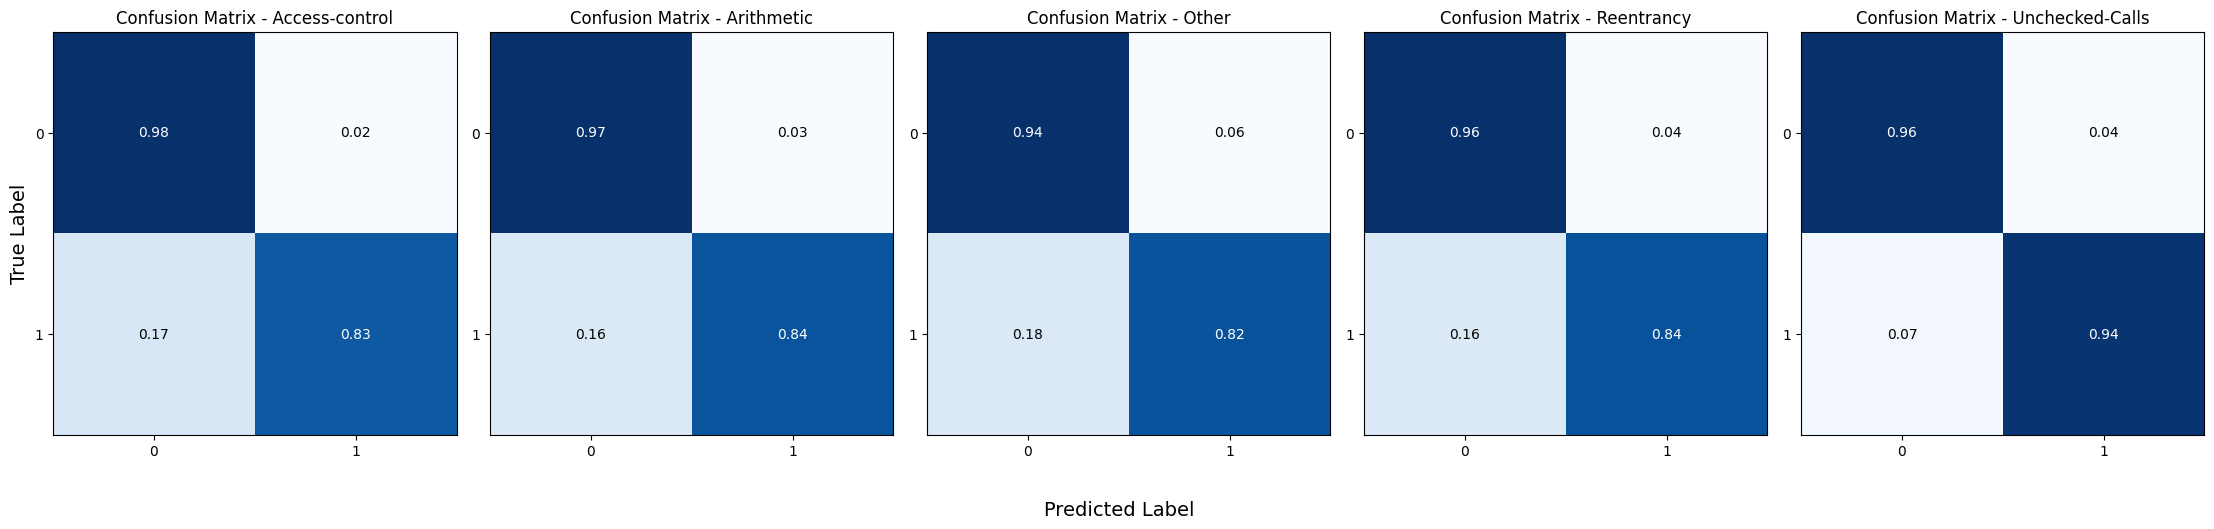
\includegraphics[width=1.05\textwidth]{../../img/CFMax3-SC.png}
        \caption{Confusion Matrices per le diverse classi del modello CodeBERT con aggregazione di tre chunk usando la funzione Max sul codice sorgente Solidity}
    \end{figure}
    

\subsubsection{Aggregazione con funzione Mean}
L'accuratezza del modello \`e del 78.97\%. Di seguito il classification report del modello:

\begin{table}[H]
    \centering
    \small
    \begin{tabular}{lcccc}
    \hline
    \textbf{Class} & \textbf{Precision} & \textbf{Recall} & \textbf{F1-Score} & \textbf{Support} \\
    \hline
    access-control & 0.89 & 0.82 & 0.85 & 2331 \\
    arithmetic & 0.89 & 0.81 & 0.85 & 2708 \\
    other & 0.83 & 0.83 & 0.83 & 4193 \\
    reentrancy & 0.92 & 0.82 & 0.86 & 4838 \\
    unchecked-calls & 0.95 & 0.93 & 0.94 & 7276 \\
    \hline
    \textbf{Micro avg} & 0.9047 & 0.8566 & 0.8800 & 21346 \\
    \textbf{Macro avg} & 0.8959 & 0.8411 & 0.8672 & 21346 \\
    \textbf{Weighted avg} & 0.9051 & 0.8566 & 0.8797 & 21346 \\
    \hline
    \end{tabular}
    \caption{Classification Report del modello con aggregazione di tre chunk usando la funzione Mean}
    \end{table}
\subsection{Analisi}
I risultati ottenuti dai modelli  sul codice sorgente Solidity riflettono tendenze simili a quelle riscontrate nel bytecode.

Innanzitutto, anche in questo caso si evidenzia un netto miglioramento del modello CodeBERT rispetto a BERT nei test iniziali con 512 token in input. Di conseguenza, \`e stato scelto di focalizzarsi sul modello CodeBERT per gli esperimenti successivi, che hanno coinvolto porzioni pi\`u ampie dei dati a disposizione.

Il modello che ha mostrato le migliori performance in termini di accuratezza e F1-Score \`e stato quello con concatenazione di tre chunk, come nel caso dei modelli addestrati sul bytecode, registrando un'accuratezza del 79,39\% e un F1 Micro dell'88,24\% sul test set. Questo risultato in F1-Score \`e condiviso con il modello che utilizza l'aggregazione di tre chunk con funzione Max, il quale ha per\`o un'accuratezza leggermente inferiore. Rispetto ai risultati ottenuti sul bytecode, l'aumento da due a tre chunk ha prodotto miglioramenti significativi in tutti gli esperimenti condotti sul codice sorgente Solidity. Questo fenomeno, potrebbe probabilmente essere dovuto alla lunghezza media del bytecode rispetto a quella del codice sorgente (ricordiamo circa 8000 contro circa 1500), quindi l'utilizzo di tre chunk di codice sorgente Solidity permette di catturare pi\`u informazioni utili rispetto al bytecode.

Nonostante il modello con concatenazione di tre chunk abbia ottenuto i migliori risultati in termini di accuratezza complessiva, \`e importante notare che in termini di recall per le singole classi, il modello con aggregazione di tre chunk e funzione Max ha dimostrato di essere il migliore per tutte le classi, tranne che per la classe ``Other". In quest'ultimo caso, il modello con aggregazione di tre chunk e funzione Mean ha ottenuto i risultati migliori.

Basandosi sull'analisi dei risultati, il modello con aggregazione di tre chunk e funzione Max \`e stato selezionato come il miglior modello per la classificazione del codice sorgente Solidity. 

\section{Risultati Stacking}
In questa sezione vengono presentati i risultati dei meta-classificatori addestrati sulle predizioni dei modelli di classificazione per il bytecode e il codice sorgente Solidity. Entrambi i modelli base selezionati utilizzano CodeBERT con aggregazione di tre chunk e funzione Max.\\

\subsection{Risultati meta-classificatori}
Di seguito, mostriamo i risultati dei meta classificatori utilizzati. Per questi modelli verranno presentate delle statistiche aggregate in quanto i risultati ottenuti sono molto simili tra loro.\\

\begin{table}[ht]
    \centering
    \resizebox{\textwidth}{!}{%
        \begin{tabular}{lccccc}
            \hline
            & \textbf{Gaussian NB} & \textbf{SVC} & \textbf{GBoost} & \textbf{Decision Tree} & \textbf{Random Forest} \\ \hline
            \textbf{Accuracy} & 0.8111 & 0.8256 & 0.8295 & 0.7959 & \textbf{0.8346} \\
            \textbf{Precision Micro} & 0.9038 & 0.9238 & 0.9252 & 0.8945 & \textbf{0.9287} \\
            \textbf{Precision Macro} & 0.8922 & 0.9153 & 0.9163 & 0.8834 & \textbf{0.9212} \\
            \textbf{Precision Weighted} & 0.9040 & 0.9235 & 0.9249 & 0.8952 & \textbf{0.9283} \\
            \textbf{Recall Micro} & \textbf{0.8944} & 0.8900 & 0.8930 & 0.8797 & 0.8939 \\
            \textbf{Recall Macro} & \textbf{0.8816} & 0.8752 & 0.8789 & 0.8653 & 0.8801 \\
            \textbf{Recall Weighted} & \textbf{0.8944} & 0.8900 & 0.8930 & 0.8797 & 0.8939 \\
            \textbf{F1 Score Micro} & 0.8990 & 0.9066 & 0.9088 & 0.8871 & \textbf{0.9110} \\
            \textbf{F1 Score Macro} & 0.8867 & 0.8947 & 0.8971 & 0.8740 & \textbf{0.9001} \\
            \textbf{F1 Score Weighted} & 0.8990 & 0.9063 & 0.9086 & 0.8872 & \textbf{0.9107} \\ \hline
        \end{tabular}
    }
    \caption{Confronto delle performance dei cinque modelli}
    \label{tab:comparison}
\end{table}
I risultati delle metriche di valutazione indicano chiaramente che il Random Forest ha ottenuto le performance pi\`u elevate in termini di Accuracy, Precision e F1 Score tra tutti i meta-classificatori testati. Tuttavia, per le metriche di Recall, il modello Gaussian Naive Bayes ha mostrato risultati marginalmente superiori.

Nonostante ci\`o, nessuno dei modelli esaminati \`e stato selezionato come il miglior candidato. Questa decisione \`e motivata dal fatto che tutti i modelli, al momento della valutazione sui dati di training, hanno mostrato segni di overfitting, fenomeno osservato in misura differente tra i vari modelli,  presentando metriche significativamente superiori rispetto a quelle ottenute sui dati di test. Il Random Forest, \`e emerso come il modello pi\`u affetto da overfitting mentre il modello di Gaussian Naive Bayes \`e risultato essere il meno affetto. Questa disparit\`a pu\`o essere facilmente attribuibile alla natura stessa dei modelli: il Random Forest essendo un modello complesso che combina un numero molto alto di alberi decisionali, \`e pi\`u incline a sovradattarsi ai dati di training rispetto ad un modello pi\`u semplice come il Gaussian Naive Bayes.\\

Nel tentativo di mitigare questo problema attraverso cross-validation e semplificando gli iperparametri dei modelli (ad esempio costruendo modelli Random Forest pi\`u piccoli e meno profondi), i risultati migliorativi non sono stati sufficienti per raggiungere un livello di generalizzazione adeguato per l'implementazione pratica del modello.

\subsection{Regressione Logistica}
Il modello di regressione logistica si \`e dimostrato il miglior classificatore ottenuto, confermando i risultati emersi nello studio di \cite{Deng}. L'accuratezza del modello \`e del 81.30\%. Di seguito il classification report del modello:

\begin{table}[H]
    \centering
    \small
    \begin{tabular}{lcccc}
    \hline
    \textbf{Class} & \textbf{Precision} & \textbf{Recall} & \textbf{F1-Score} & \textbf{Support} \\
    \hline
    access-control & 0.91 & 0.82 & 0.86 & 2331 \\
    arithmetic & 0.90 & 0.85 & 0.88 & 2708 \\
    other & 0.85 & 0.87 & 0.86 & 4193 \\
    reentrancy & 0.91 & 0.87 & 0.89 & 4838 \\
    unchecked-calls & 0.96 & 0.94 & 0.95 & 7276 \\
    \hline
    \textbf{Micro avg} & 0.9144 & 0.8835 & 0.8987 & 21346 \\
    \textbf{Macro avg} & 0.9074 & 0.8678 & 0.8868 & 21346 \\
    \textbf{Weighted avg} & 0.9147 & 0.8835 & 0.8986 & 21346 \\
    \hline
    \end{tabular}
    \caption{Classification Report per il modello di Regressione Logistica}
\end{table}

\begin{figure}[H]
    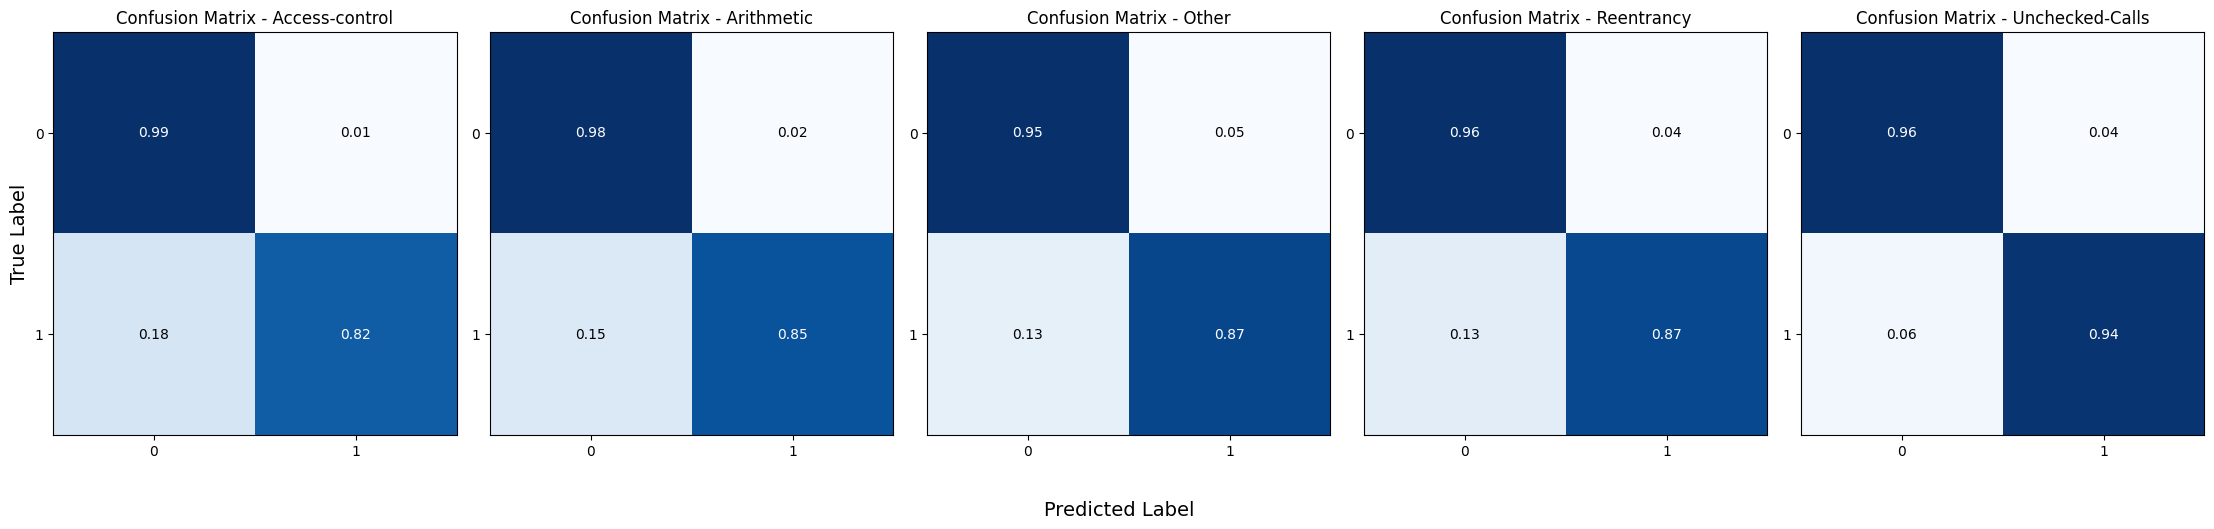
\includegraphics[width=1.05\textwidth]{../../img/CF-LR.png}
    \caption{Confusion Matrices per le diverse classi del modello Logistic Regression}
\end{figure}

Rispetto agli altri modelli utilizzati come meta-classificatori, la regressione logistica mostra miglioramenti significativi in tutte le metriche di valutazione, particolarmente evidenti nella precisione e nel recall senza mostrare segni di overfitting. L'unica eccezione \`e rappresentata dal recall per la classe access-control, la quale \`e la classe minoritaria in questo contesto di classificazione.

Inoltre, a differenza degli altri modelli utilizzati come meta-classificatori, la regressione logistica non mostra segni di overfitting. Questo suggerisce che un approccio pi\`u semplice possa essere pi\`u adatto per questo tipo di problemi di classificazione.



\section{Risultati Gemini}

In questa sezione verranno presentati i risultati ottenuti utilizzando le API del modello Gemini, valutati secondo le metriche descritte in precedenza.\\
L'accuratezza del modello \`e del 27.54\%. Di seguito il classification report del modello:


\begin{table}[H]
    \centering
    \small
    \begin{tabular}{lcccc}
    \hline
    \textbf{Class} & \textbf{Precision} & \textbf{Recall} & \textbf{F1-Score} & \textbf{Support} \\
    \hline
    access-control & 0.24 & 0.04 & 0.06 & 171 \\
    arithmetic & 0.19 & 0.04 & 0.07 & 198 \\
    other & 0.28 & 0.49 & 0.36 & 282 \\
    reentrancy & 0.41 & 0.08 & 0.14 & 364 \\
    unchecked-calls & 0.45 & 0.20 & 0.28 & 475 \\
    \hline
    \textbf{Micro avg} & 0.3271 & 0.1872 & 0.2382 & 1490 \\
    \textbf{Macro avg} & 0.3137 & 0.1706 & 0.1800 & 1490 \\
    \textbf{Weighted avg} & 0.3490 & 0.1872 & 0.2056 & 1490 \\
    \hline
\end{tabular}
\caption{Classification Report del modello Gemini}
\end{table}

\begin{figure}[H]
    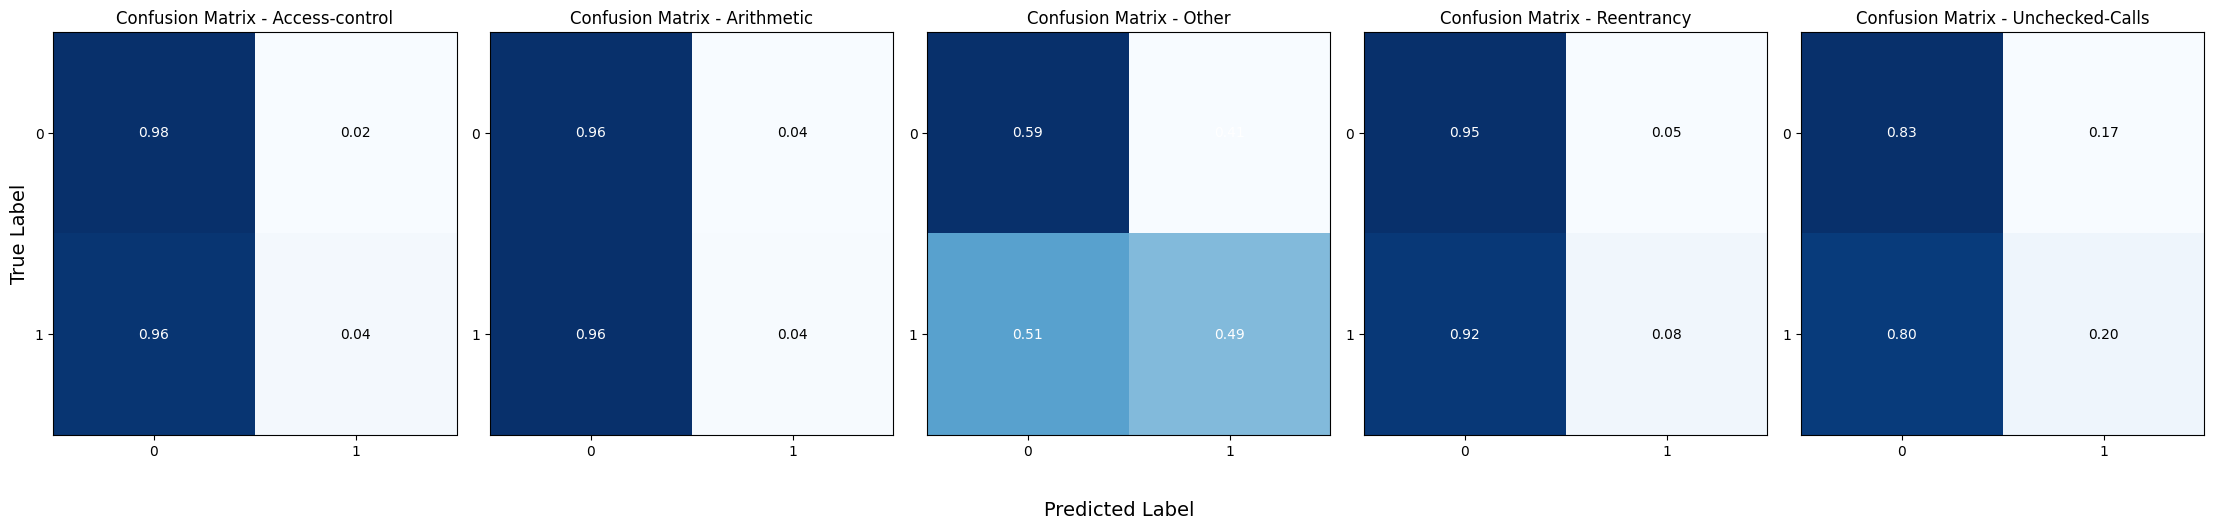
\includegraphics[width=1.05\textwidth]{../../img/CF-Gemini.png}
    \caption{Confusion Matrices per le diverse classi del modello Gemini}
\end{figure}
    I risultati del modello Gemini indicano una performance complessivamente scarsa nelle metriche di valutazione. L'Accuracy del 27.54\% evidenzia che meno di un terzo delle previsioni del modello sono corrette. La Precision micro del 32.71\% indica che solo un terzo delle istanze classificate positivamente sono effettivamente corrette, mentre la Precision macro e weighted, rispettivamente 31.37\% e 34.90\%, mostrano variazioni nella performance tra le diverse classi. Il Recall micro dell'18.72\% suggerisce che il modello riesce a identificare meno di un quinto delle istanze rilevanti, con valori macro e weighted simili, indicando che il modello ha difficolt\`a a catturare tutte le istanze corrette. L'F1 Score, che bilancia precision e recall, \`e basso in tutte le versioni, suggerendo un compromesso non soddisfacente tra la capacit\`a del modello di evitare falsi positivi e falsi negativi.\\
    Analizzando le performance per classe, si osserva che il modello ha ottenuto risultati migliori solo per la classe ``Other", con un Recall del 49\%. Interessante \`e il risultato per la classe ``reentrancy", una delle vulnerabilit\`a pi\`u comuni, che ha ottenuto un Recall dell'8\%. Questo evidenzia una specifica difficolt\`a del modello nel riconoscere questa particolare categoria di vulnerabilit\`a.\\
    Complessivamente, il modello Gemini non ha raggiunto risultati soddisfacenti nella classificazione delle vulnerabilit\`a del codice sorgente. Le metriche di valutazione indicano la necessit\`a di miglioramenti significativi per rendere il modello pi\`u affidabile e preciso nella sua capacit\`a di identificare correttamente le vulnerabilit\`a del codice sorgente Solidity, mostrando la necessit\`a di avere modelli ad hoc per task specifici e complessi come questo.
\end{document}
